\documentclass{standalone}
\usepackage{tikz}
\usepackage{verbatim}
\usetikzlibrary{positioning}
\begin{document}
\pagestyle{empty}
  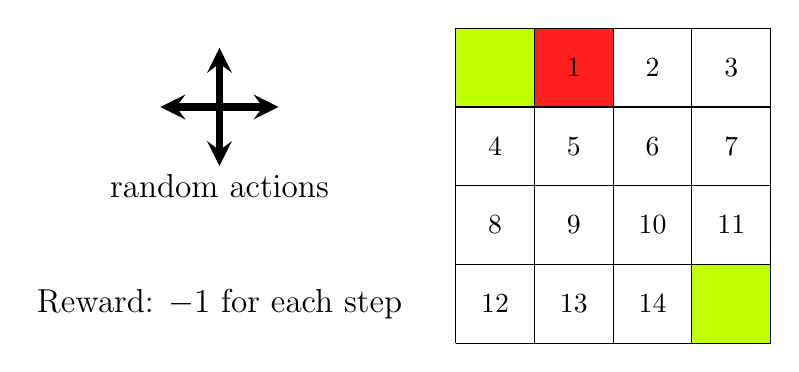
\begin{tikzpicture}
    \draw[stealth-stealth, line width=1 mm] (-3.75, 3) -- (-2.25, 3);
    \draw[stealth-stealth, line width=1 mm] (-3, 2.25) -- (-3, 3.75);
    \node at (-3, 2) {\large random actions};
    \node at (-3, 0.5) {\large Reward: $-1$ for each step};
    \fill[lime] (0, 3) rectangle (1,4);
    \fill[lime] (3, 0) rectangle (4,1);
    % Top row.
    \fill[red!88] (1, 3) rectangle (2,4);
    \node at (1.5, 3.5) {1};
    \node at (2.5, 3.5) {2};
    \node at (3.5, 3.5) {3};
    % Second frop top row.
    \node at (0.5, 2.5) {4};
    \node at (1.5, 2.5) {5};
    \node at (2.5, 2.5) {6};
    \node at (3.5, 2.5) {7};
    % Second from bottom row.
    \node at (0.5, 1.5) {8};
    \node at (1.5, 1.5) {9};
    \node at (2.5, 1.5) {10};
    \node at (3.5, 1.5) {11};
    % Bottom row.
    \node at (0.5, 0.5) {12};
    \node at (1.5, 0.5) {13};
    \node at (2.5, 0.5) {14};
    \draw[step=1.0,black] (0,0) grid (4, 4);
  \end{tikzpicture}
\end{document}